%%%%%%%%%%%%%%%%%%%%%%%%%%%%%%%%%%%%%%%%%%%%%%%%%%%%%%%%%%%%%%%%%%%%%%%%%%%%%
%	e-Yantra, IIT-Bombay

%	Document Author: Saurav Shandilya
%	Date: 16-August,2012
%	Last Editted by: Saurav
%   Date Last updated: 31-05-2016 

%%%%%%%%%%%%%%%%%%%%%%%%%%%%%%%%%%%%%%%%%%%%%%%%%%%%%%%%%%%%%%%%%%%%%%%%%%%%%

\documentclass[11pt,a4paper]{article}

\usepackage{graphicx}
\usepackage[utf8]{inputenc}
\newcommand\tab[1][1cm]{\hspace*{#1}}
\usepackage{listings}
\usepackage{color}
 \usepackage{hyperref}
\definecolor{codegreen}{rgb}{0,0.6,0}
\definecolor{codegray}{rgb}{0.5,0.5,0.5}
\definecolor{codepurple}{rgb}{0.58,0,0.82}
\definecolor{backcolour}{rgb}{0.95,0.95,0.92}
 
\lstdefinestyle{mystyle}{
    backgroundcolor=\color{backcolour},   
    commentstyle=\color{codegreen},
    keywordstyle=\color{magenta},
    numberstyle=\tiny\color{codegray},
    stringstyle=\color{codepurple},
    basicstyle=\footnotesize,
    breakatwhitespace=false,         
    breaklines=true,                 
    captionpos=b,                    
    keepspaces=true,                 
    numbers=left,                    
    numbersep=5pt,                  
    showspaces=false,                
    showstringspaces=false,
    showtabs=false,                  
    tabsize=2
}
 
\lstset{style=mystyle}
 
\title{\textbf{\Huge{Galileo Board}}\vspace{6mm}\\Basic Tutorial}
\author{Sanket R. Bhimani}
\date{\today}

\begin{document}
	\maketitle
	\newpage
	\tableofcontents
	\newpage
	\section{Tutorial Name:}
	\begin{center}\huge{"Basic Tutorial For Galileo Board"}\end{center}
	\tab{This tutorial will help you to do basic interfacing with Galileo board. This board is new to market. So, you will not get enough resources to complete your tasks.}

    \vspace{15mm}
	\section{Prerequisites:}
	\vspace{1cm}
		\begin{itemize}
	    \item 	Basic knowledge of Linux OS because we will run Linux on Galileo board. 
	    \item 	Basic Arduino programming. 
	    \item 	what is SSH
	    \item	read Galileo from “Sign Language Interpreter” tutorial, so you get knowledge about installing Linux on the Galileo board.
	\end{itemize}
    \newpage
    \section{Requirement}
	\vspace{1cm}
	\begin{itemize}
	    \item Hardware Requirement:
	    \begin{itemize}
	        \item Galileo Board
	        \item LEDs
	        \item Servo Motors
	        \item Connecting wires
	        \item LAN cable or WIFI module(for connecting board with PC)
	        \item 5V power supply
            \item SD card of minimum 8 GB
	    \end{itemize}
	    \vspace{1cm}

	    \item Software Requirement:
	    \begin{itemize}
	        \item Python editor
	        \item Leap sdk
	        \item SSH Client
            \item Arduino IDE
	        \item various library
	        \item SSH Client
	        \item Wireshark(optional)
	    \end{itemize}
	\end{itemize}
	\newpage
    \section{Theory and Description}
	\vspace{.3cm}
    \begin{itemize}
		\item Galileo board can be used in two ways :
        \begin{itemize}
			\item As an Arduino (IDE is also same)
            \item By installing a particular OS on it. 
Board supports three OS: Linux, Windows IOT and OSX
\end{itemize}
	\end{itemize}
    \tab{IOT feature is also available for both modes. This implies that the board can be connected to the Internet without installing any OS.}
    
    \vspace{1cm}
    \begin{figure}
	\includegraphics[width=\linewidth]{7.png}
    \caption{Pin configuration}
    \end{figure}
    \newpage
    \tab{For using Galileo board from Arduino IDE no extra fuctions are required as all the things are same. We just need to select Galileo in board option. (Refer to Figure 1)}\\
    \vspace{.3cm}\\
\textbf{Tools -) Board -) Intel Galileo}
 \vspace{1cm}
	\begin{figure}
  
  \includegraphics[width=\linewidth]{8.png}
  \caption{Arduino IDE selecting board}
  
\end{figure}
	\vspace{.3cm}\\
    
    Then choose the appropriate port number from:\\
\textbf{Tools -) Port}
\newpage

\newpage
\textbf{\huge{Installation of Linux image in Galileo board:}}
	\vspace{1cm}\\
	\tab{In Galileo board, we can install Linux, windows IOT or os x. So the interface with board become easy. Here we will use Linux image. For that, we need to write Linux image on the sd card. From sd card, Galileo board will boot.}\\
	\vspace{.5cm}\\
	\textbf{\Large{So How to prepare sd card???}}\\
	\vspace{.3cm}\\
	\textbf{Step 1:}\\
	Download Linux image from this location.\\
	\url{https://downloadmirror.intel.com/26028/eng/iot-devkit-prof-dev-image-galileo-20160525.zip}\\
	You will get one zip file extract it. You will find one ‘.direct’. You need to write this into sd card\\
	\vspace{.3cm}\\
	\textbf{Step 2:}\\
	Download this software from this location,\\
 \url{http://download.softpedia.com/dl/d5a643aad00816ee735372c2d530a1a2/57584b56/100173006/software/cd_dvd_tools/Win32DiskImager-0.9.5-binary.zip}\\
this will be helpful for writing an image in sd card.\\
\vspace{.3cm}\\
\begin{figure}
	\includegraphics[width=\linewidth]{1.png}
    \caption{Win32 Disk Image windows}
    \end{figure}
\vspace{.3cm}\\
Select Image File which you have downloaded earlier in ‘Image File’ tab(‘.direct’ file)\\
Select sd card in ‘Device tab’\\
Now click on ‘Write’ button, it will take some time. And wait until write process completes\\
\vspace{.3cm}\\
	\textbf{Step 3:}\\
	\vspace{.3cm}\\
	\tab{Now insert sd card in galileo board and connect LAN cable with your PC and galileo board. Now connect the power supply with galileo board.}

\tab{now the board will automatically boot.}
\tab{There will be blinking LED near sd card port. Wait until it stops lighting. Because it shows IO related sd card. So, when it become stop, IO related sd card is also stopped so the booting process is completed.}
\tab{Now you need to find  the IP address of your board. For that, you can use any network packet tracer software like Wireshark, ettercap or any other.}

\tab{I am using Wireshark.}

\tab{Now open Wireshark select ethernet as a network adapter. It will start tracing all packet data on ethernet. But here on an ethernet network, there is only two devices are there your PC and board. So there is only two IP address data. (ignore IPs with 255, 251, 224 and more than 200 value in last two part like 192.168.0.255 or 255.255.255.0 ) so find your PC IP address using this command }\\
\vspace{1cm}
\begin{lstlisting}
ipconfig (for windows)}
ifconfig (for Linux)}
\end{lstlisting}
\vspace{1cm}
\tab{Now another IP showing on Wireshark is your board IP. }
\vspace{.3cm}\\
\begin{figure}
	\includegraphics[width=\linewidth]{2.png}
    \caption{CMD for your IP address}
    \end{figure}
\vspace{.3cm}\\
Your Wireshark windows:\\
\vspace{.3cm}\\
\begin{figure}
	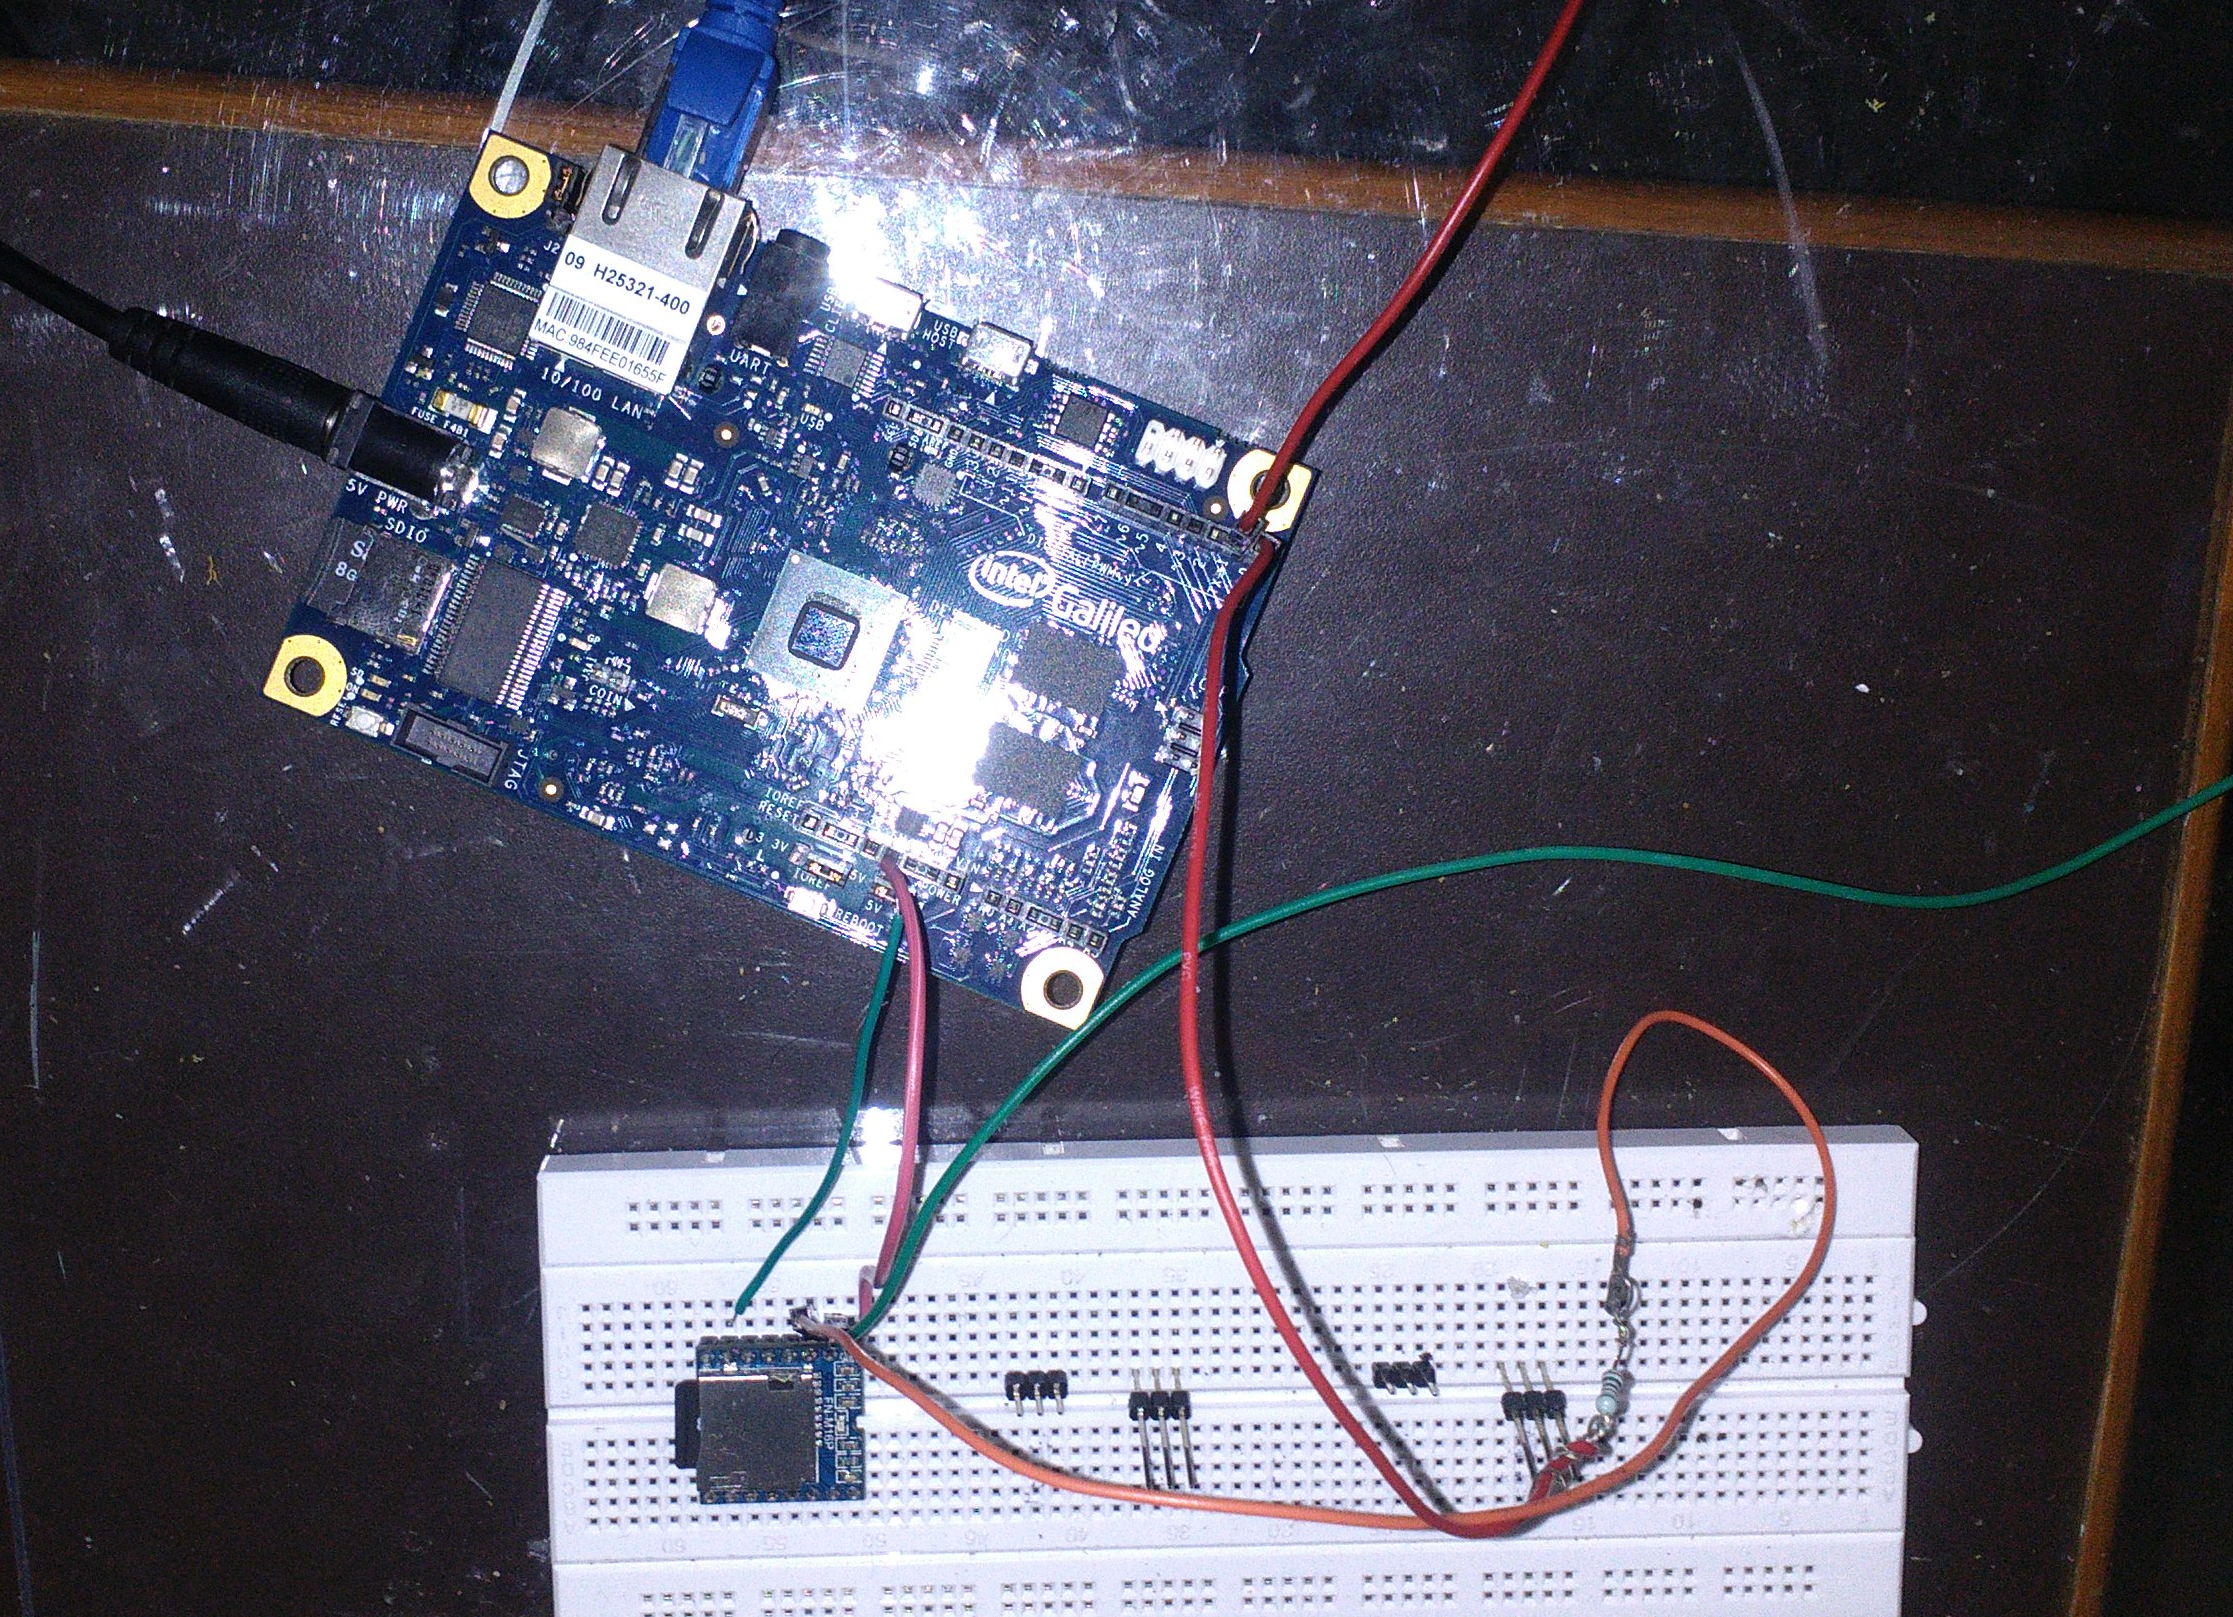
\includegraphics[width=\linewidth]{3.png}
    \caption{Wireshark windows for board IP}
    \end{figure}
\newpage
	\textbf{Step 3:}\\
	\vspace{.3cm}\\
	Now, from any SSH client make connection with board and use. :?)\\
(I’m using Bitvise SSH client)\\
Enter IP address and username: root there is no password.\\
\vspace{.3cm}\\
\begin{figure}
	\includegraphics[width=\linewidth]{4.png}
    \caption{SSH client window}
    \end{figure}
\vspace{.3cm}\\
Click on login, and wait. Now two windows will open one for terminal and another for file transfer.
Your board is ready! :?)
  \vspace{.3cm}\\
\begin{figure}
	\includegraphics[width=\linewidth]{5.png}
    \caption{SSH client file transfer window}
    \end{figure}
\vspace{.3cm}\\
\begin{figure}
	\includegraphics[width=\linewidth]{6.png}
    \caption{SSH client terminal window}
    \end{figure}
\newpage
\textbf{\huge{Basic interface with GPIO pins:}}
\tab{Most of GPIO capabilities are done through Linux Sysfs. Means board can be controlled by file based I/O operation. Means Galileo linux os gives an interface to controle GPIO pins through something like file system. So using that we can get inputs and also gives outputs or generate PWM signals.}\\
\tab{For that there is some steps tobe followed,}\\
\begin{itemize}
	\item First you need to export that pin
    \item \begin{itemize}
	\item Defining the pin number which you are using 
\end{itemize}

	\item Then set direction 'in' or 'out'
    \item \begin{itemize}
	\item Define that you are using it as input or output
\end{itemize}

	\item GPIO Port Drive Configuration: ‘pullup’, ‘pulldown’, ‘strong’ or ‘hiz’ (Optional)
    \item \begin{itemize}
	\item Define the intensity.
\end{itemize}

	\item Read or write value

\end{itemize}
\newpage
\textbf{Steps to be followed to blink/glow LED:}\\

\begin{lstlisting}
root@Galileo:~#echo -n "24" > /sys/class/gpio/export
root@Galileo:~#echo -n "out"> /sys/class/gpio/gpio24/direction
root@Galileo:~#echo -n "strong" > /sys/class/gpio/gpio24/drive
root@Galileo:~#echo -n "1" > /sys/class/gpio/gpio24/value
\end{lstlisting}
\vspace{.3cm}
\begin{figure}
	\includegraphics[width=\linewidth]{9.png}
    \caption{LED connection}
    \end{figure}

\vspace{.3cm}
\tab{Here 27 is allocated for digital pin 6 so connect your LED at digital pin number 70}
\newpage
Here is the chart for mapping with on board pin to linux SYSFS system for GPIO\\

\begin{figure}
	\includegraphics[width=\linewidth]{10.png}
    \caption{Table for GPIO pin and SYSFS pin}
    \end{figure}
   Here in setting column you need to set given value to use that pin.\\
   This way you can perform any tasks like,
   \begin{itemize}
\item 	Digital input
\item 	Digital output
\item	Analog input
\item	PWM singal
\item	SPI I/O
\item	I2C I/O
\item	Fast I/O

\end{itemize}
\newpage
\large{\textbf{Digital Input:}}\\
\vspace{.3cm}\\
It will help you to take input from digital pins\\

\begin{lstlisting}
root@Galileo:~#echo -n "27" > /sys/class/gpio/export
\end{lstlisting}
here 27 is gpio pin number\\

and /sys/class/gpio is a path of something like file from whch you can access gpio pins\\
\begin{lstlisting}
root@Galileo:~#echo -n "in"> /sys/class/gpio/gpio27/direction
\end{lstlisting}
'in' means using as input\\
\begin{lstlisting}
root@Galileo:~#cat /sys/class/gpio/gpio27/value
1
\end{lstlisting}

reading the value 1\\
\vspace{.3cm}

This will give you the value input on digital pin 7 in form of 0 or 1\\
\vspace{1cm}\\

\large{\textbf{Digital Output:}}\\
\vspace{.3cm}\\
It will help you to give output to digital pins\\
\begin{lstlisting}
root@Galileo:~#echo -n "27" > /sys/class/gpio/export
\end{lstlisting}
here 27 is gpio pin number\\

and /sys/class/gpio is a path of something like file from whch you can access gpio pins\\
\begin{lstlisting}
root@Galileo:~#echo -n "out"> /sys/class/gpio/gpio27/direction
\end{lstlisting}
'out' means use as output\\
\begin{lstlisting}
root@Galileo:~#echo -n "strong" > /sys/class/gpio/gpio27/drive
\end{lstlisting}.
set intensity of pin 7
\newpage
\begin{lstlisting}
root@Galileo:~#echo -n "1"> /sys/class/gpio/gpio27/value
\end{lstlisting}
set value\\
\vspace{1cm}\\
\large{\textbf{Analog Input:}}\\
\vspace{.3cm}\\
This will helps you to take input from analog pin.\\
If we want to take input from analog pin 0 we need to set GPIO37 = 0 (as shown in figure)\\
\begin{lstlisting}
root@Galileo:~#echo -n "37" > /sys/class/gpio/export
root@Galileo:~#echo -n "out"> /sys/class/gpio/gpio37/direction
root@Galileo:~#echo -n "0"> /sys/class/gpio/gpio37/value
\end{lstlisting}.
we need to do some setting for take input from A0 as per figure: 10\\
And now read the value from A0 pin at this way,\\
\begin{lstlisting}
root@Galileo:~#catsys/bus/iio/devices/iio\:device0/in_voltage0_raw
2593
\end{lstlisting}



\vspace{.3cm}
\large{\textbf{Generating PWM signal:}}
\vspace{.1cm}\\
Here is the mapping with digital pin number and PWM SYSFS gpio no.\\
\vspace{.3cm}
\begin{figure}
	\includegraphics[width=\linewidth]{11.png}
    \caption{Digital pin number with PWM channel number}
    \end{figure}
    \vspace{.3cm}
    Now, If we want to generate PWM signal of period 1 millisecond and duty cycle 50\% then follow this command,
    \vspace{.3cm}
\begin{lstlisting}
root@Galileo:~#echo -n "3" > /sys/class/pwm/pwmchip0/export
\end{lstlisting}
To enable a PWM on a port write "1" to a corresponding enable file. To disable a port write "0".\\

\begin{lstlisting}
root@Galileo:~#echo -n "1">/sys/class/pwm/pwmchip0/pwm3/enable
\end{lstlisting}
To set a PWM period write period in nanoseconds to period file. In example below it is set to 1000000 nanoseconds or 1 millisecond:\\
\begin{lstlisting}
root@Galileo:~#echo -n "1000000">/sys/class/pwm/pwmchip0/pwm3/period
\end{lstlisting}.

To set a PWM duty cycle write its length in nanoseconds to duty\_cycle file. In example below we set duty cycle to 50\% (500000/1000000*100\%):


\begin{lstlisting}
root@Galileo:~# echo -n"500000" > /sys/class/pwm/pwmchip0/pwm3/duty_cycle
\end{lstlisting}

\vspace{.3cm}
\large{\textbf{Fast I/O:}}
\vspace{.1cm}\\
\tab{Galileo supports fast I/O on digital pins 2 and 3 which can be connected using multiplexer directly to Intel Quark X1000}\\

\vspace{.3cm}
Normally, we are not developing system using this way, we are using some library like mraa, wiringx86, jonny-five or many others.

\newpage
\textbf{\huge{Wiring-x86:}}\\
\vspace{.1cm}\\
\tab{This library is for python programming}\\
\tab{This library do same thing like normal GPIO SYSFS. But here ready to us functions which will be helpful for changing values in file so it will be more easy to work with this library.}\\
\tab{But still some thing we can’t do with library, like running a servo. Because for running servo we need to generate PWM signal of 20 ms period and 0-2 ms duty cycle. Library accepts PWM signal values in nano seconds range.PWM signal values in range of millisecond
}\\
\tab{seconds exceeds the maximum range of input values.}\\
\tab{So, in this case this library fails to woks. But still, for prforming small taskes like running leds or any other GPIO process we can use this library.}\\
\tab{This library woks with,}
\begin{itemize}
\item Intel Galileo Board
\item Intel Galileo Board Gen 2
\item Intel Edison Board
\end{itemize}
\vspace{.2cm}
\tab{Here are some functions which will be use to interfaceing with GPIO:}\\
\begin{itemize}
\item	GPIO()
\begin{itemize}
\item	It’s a constructer, From it we can create object of GPIO class it accepts one argument “debug=boolean” means if debug=True, it will be run in debuging mode mean you can get descrption of every task and log. And if it False it will work in normal mode
\item Example:
\begin{lstlisting}
from wiringx86 import GPIOEdison as GPIO
gpio = GPIO()
	#or
gpio = GPIO(debug=False)
\end{lstlisting}

\end{itemize}
\item	gpio.analogRead()
\begin{itemize}
\item	-	here gpio is object. This function is used to read data from anaog pins. It accepts one argument which is the anlog pin number on board. And it’s returns digital representation with 10 bits resolution. Means 0 to 1023
\item Example:
\begin{lstlisting}
value = gpio.analogRead(analogpin) 
\end{lstlisting}

\end{itemize}
\item 	gpio.analogWrite()
\begin{itemize}
\item	This function is used to write analog data on pins. But you can’t do that right!!! So, this function used for writing value in PWM pins. It accepts two perameters one is pin number and second is value. Value will be between 0 to 255. Means at 255 complete signal will be gone means always 1 and at 0 always 0.


\end{itemize}
\item	gpio.cleanup()
\begin{itemize}
\item	Do a general cleanup. Close all open handlers for reading and writing. Unexport all exported GPIO pins and unexport all exported. Calling this function is not mandatory but it’s recommended once you are finished using the library and if it is beingused with a larger application that runs for a long period of time. 
\item Example:
\begin{lstlisting}
gpio.cleanup() 
\end{lstlisting}

\end{itemize}
\item 	gpio.digitalRead()
\begin{itemize}
\item	Read the state of digital pin meand itwill be used totakeinput from digital pin. It accepts one aguments which is pin number.
\item Example:
\begin{lstlisting}
state = gpio.digitalRead(pin) 
\end{lstlisting}

\end{itemize}
\item 	gpio.digitalWrite()
\begin{itemize}
\item	this is used to give output from digital pin. It accepts two arguments one is pin number and second is state (states are as shown earlier in SYSFS.)
\item Example:
\begin{lstlisting}
gpio.digitalWrite(13, gpio.HIGH) 
\end{lstlisting}

\end{itemize}
\item 	gpio.pinMode()
\begin{itemize}
\item	this is used for setting the pin mode. Pin modes are shown  below,
\begin{itemize}
\item OUTPUT: pin used as output. Use to write into it.
\item INPUT: pin used as input (high impedance). Use to read from it.
\item INPUT\_PULLUP: pin used as input (pull up resistor). Use to read from it.
\item INPUT\_PULLDOWN: pin used as input (pull down resistor). Use to read from it.
\item ANALOG\_INPUT: pin used as analog input (ADC).
\item PWM: pin used as analog output (PWM).
\end{itemize}
\item This function accepts two arguments one is pin number and another is string specified pin mode
\item Example:
\begin{lstlisting}
gpio.pinMode(pin, gpio.OUTPUT)
\end{lstlisting}

\end{itemize}
\item 	gpio.setPWMPeriod()
\begin{itemize}
\item	this is used for setting the PWM period. And it accepts two argument one is pin and another is PWM period value


\end{itemize}
\end{itemize}
\tab{Still this library is not suitable for servo. Because, basically it uses SYSFS GPIO system and there we can not set 20 ms as time period of PWL signal so we cannot drive servo using this library
}
\newpage
\textbf{\huge{Wiring-x86:}}\\
\vspace{.1cm}\\
\tab{This library is not based on SYSFS. It works independantly so it is very good and easy to use. This library supports many boards like Galileo Gen1 and Gen2, Edison, Raspberry Pi, Banana Pi and many more.}\\
\tab{We will keep the focus on Galileo board.}\\
\vspace{.1cm}
\textbf{Installation:}\\
\vspace{.1cm}
Normally it’s comes with OS. But still if you want to install,\\
\vspace{.1cm}
\begin{lstlisting}
echo"srcmraa-upm http://iotdk.intel.com/repos/3.0/intelgalactic/opkg/i586"> /etc/opkg/mraa-upm.conf
opkg update
opkg install mraa
\end{lstlisting}
\vspace{.1cm}
\tab{use this command on board with internet connection on board}\\
\tab{this library is avilable for many plateforms like python, c/c++, node.js and java.}\\
\begin{itemize}
\item Analog Input:
\begin{lstlisting}
x = mraa.Aio(0)
print (x.read())
print ("%.5f" % x.readFloat())
\end{lstlisting}
\tab{here mraa.Aio() gives the object of analog pin ‘0’. Using that object you can read the valus of that analog pin.}\\
\tab{Using this x.read() you can read value in integer. But using x.readFloat() function you can read values more precisely.}\\
\item Digital Output: 
\begin{lstlisting}
x = mraa.Gpio(8)
x.dir(mraa.DIR_OUT)
x.write(1)
\end{lstlisting}
\tab{here mraa.Gpio(8) gives object of digital pin ‘8’. Using that object you can write high or low voltage on pin number ‘8’}\\
\tab{and x.dir() specifies the direction means input or output. mraa.DIR\_OUT specifies output and mraa.DIR\_IN specifies input. And x.write() writes the values on that pin.}\\
\newpage
\item Digital Input:
\begin{lstlisting}
x=mraa.Gpio(8)
x.dir(mraa.DIR_IN)
a = x.read()
\end{lstlisting}
\tab{this way we can read from digital pin 8. And returns 1 or 0}\\
\item PWM:
\begin{lstlisting}
x = mraa.Pwm(3)
x.period_us(1000)
x.enabe(True)
x.write(.5)
\end{lstlisting}
\tab{here mraa.Pwm(3) specifies pwm pin and using period\_us() specifies the period of pwm signal and input is in micro second. There is period\_ms() is also available for input in milliseconds. And using enable(True) starts sending pwm signal and with enable(False).}\\
\tab{And write() method use to specify duty cycle. The input in in range of 0 to 1 1 secifies 100\% duty cycle and 0 specifies 0\% duty cycle.}
\item UART:
Reciver:
\begin{lstlisting}
u = mraa.Uart(0)
u.setBaudRate(9600)
u.setMode(8, mraa.UART_PARITY_NONE, 1)
while True:
	if u.dataAvailable():
		data_byte = u.readStr(1)
		print(data_byte)
\end{lstlisting}
\tab{here mraa.Uart(0) gives uart object and 0 is init perameter. And using setBaudRate() method we can set baudrate. And using setMode() method have four perameters in sequnce:}
\begin{itemize}
\item The UART context
\item data bits
\item Parity bit setting
\item stop bits

\end{itemize}
\tab{if you do not specifies this method it will take default value which is suitable for most of the cases.}\\
\tab{And method dataAvailabe() we can get knowledge weather more bits available or not. And using readStr() method we can get content in string data type.}\\
\vspace{.2cm}\\
Sender:
\begin{lstlisting}
u = mraa.Uart(0)
u.setBaudRate(9600)
u.setMode(8, mraa.UART_PARITY_NONE, 1)
msg_b = bytearray("Hello, mraa byte array!", "ascii")
u.write(msg_b)
u.flush()
msg = "Hello, mraa byte array!"
u.writeStr(msg)
u.flush()
\end{lstlisting}
\tab{here mraa.Uart(0) gives uart object and 0 is init perameter. And using setBaudRate() method we can set baudrate. And using setMode() method have four perameters in sequnce:}
\begin{itemize}
\item The UART context
\item data bits
\item Parity bit setting
\item stop bits

\end{itemize}
\tab{
here u.write() send data but it accepts input only in byte array. But here writeStr() method is also avilabe to dirct input into string.}\\

\end{itemize}
\newpage
\section{Prerequisites:}
	\vspace{1cm}
    \textbf{\Large{Experiment 1: Basic example to use Galileo board without loading any OS:}}\\
    \vspace{.1cm}
    This experiments shows how to start led using arduino IDE:\\
    First follow this steps:\\
    \begin{itemize}
\item select board
\item select port
\item connect board with laptop
\end{itemize}
\vspace{.1cm}
\begin{lstlisting}
/*
  Blink
  Turns on an LED on for one second, then off for one 	second, repeatedly on ppin nuumber 13
*/
void setup() {
  pinMode(13, OUTPUT);			//defining the pin as output
}
void loop() {
  digitalWrite(13, HIGH);			//writing value HIGH
  delay(1000);					//delay of one second
  digitalWrite(13, LOW);			//writeing low value
  delay(1000)					//delay of one second
}

\end{lstlisting}

\textbf{Connection:}
See figure: 12
\begin{figure}
	\includegraphics[width=\linewidth]{9.png}
    \caption{LED connection}
    \end{figure}
    
\vspace{1cm}
    \textbf{\Large{Experiment 2: Starting LED using SYSFS interface of Linux OS of Galileo board:}}\\
    \vspace{.1cm}\\
    This experiments shows how to start led using SYSFS
\begin{lstlisting}
root@Galileo:~#echo -n "39" > /sys/class/gpio/export
root@Galileo:~#echo -n "out"> /sys/class/gpio/gpio39/direction
\end{lstlisting}
select 13 pin as output
\begin{lstlisting}
root@Galileo:~#echo -n "strong" >/sys/class/gpio/gpio39/drive
\end{lstlisting}
set intensity	
\begin{lstlisting}
root@Galileo:~#echo -n "1" > /sys/class/gpio/gpio39/value
\end{lstlisting}
write value\\

\textbf{Connection:}
See figure: 12
\vspace{1cm}
    \textbf{\Large{Experiment 3: Starting LED using wiring-x86 library:}}\\
    \vspace{.1cm}\\
   This experiments shows how to start led for 3 second using wiring-x86 library 
\begin{lstlisting}
from wiringx86 import GPIOGalileo as GPIO
import time
gpio = GPIO(debug=False)			#create object with debug = false so  no log will be displayed
gpio.pinMode(13, gpio.OUTPUT)		#set pin 13 as output
gpio.digitalWrite(13, gpio.HIGH)		#write 1 in pin 13
time.sleep(1)					#delay of one second 
gpio.digitalWrite(13,gpio.LOW)		#write 0 in pin 13
gpio.cleanup()					#undefine all the pins
\end{lstlisting}


\textbf{Connection:}
See figure: 12\\
\vspace{1cm}
    \textbf{\Large{Experiment 4: Starting LED using MRAA library:}}\\
    \vspace{.1cm}\\
   This experiments shows how to start led for 3 second using wiring-x86 library 
\begin{lstlisting}
import mraa
x = mraa.Gpio(13)			#get objetc of pin 13
x.dir(mraa.DIR_OUT)			#set as output pin
x.write(1)				#set value HIGH
time.sleep(1)				#delay of 1 second
x.write(0)				#set value low
\end{lstlisting}

\textbf{Connection:}
See figure: 12

\newpage
    \textbf{\Large{Experiment 5: Send data on UART:}}\\
    \vspace{.1cm}\\
   This experiment shows how to send data on UART port.
\begin{lstlisting}
import mraa
import sys
sys.stdout.write("Initializing UART...")
u=mraa.Uart(0)						#get object of uart
u.setBaudRate(115200)				#set baudrate
msg_b = bytearray("Hello, mraa byte array!", "ascii")	#convert string to byte array
u.write(msg_b)					#send data
u.flush()				
msg_s = "Hello, mraa string!"
u.writeStr(msg_s)			#send direct to string
\end{lstlisting}

\textbf{Connection:}
See figure: 13
\begin{figure}
	\includegraphics[width=\linewidth]{12.png}
    \caption{UART connection}
    \end{figure}
   \newpage
       \textbf{\Large{Experiment 6: Receive data from UART:}}\\
    \vspace{.1cm}\\
   This experiment shows how to send data on UART port.
\begin{lstlisting}
u=mraa.Uart(0)
u.setBaudRate(115200)
while True:															#always keep watching if data is avilable
if u.dataAvailable():
		data_byte = u.readStr(1)				#read data if avilable
		print(data_byte)

\end{lstlisting}

\textbf{Connection:}
See figure: 13\\
\vspace{1cm}

        \textbf{\Large{Experiment 7: Generate PWM using mraa library:}}\\
    \vspace{.1cm}\\
   This experiments shows how to generate PWM signal.
\begin{lstlisting}
import mraa
import time
x = mraa.Pwm(3)			#select pwm pin
x.period_ms(20)			#set time period
x.enable(True)			#start signaling
x.write(0.05)			#write duty cycle
\end{lstlisting}

\textbf{Connection:}
See figure: 14\\
\begin{figure}
	\includegraphics[width=\linewidth]{13.png}
    \caption{servo connection}
    \end{figure}
    \vspace{1cm}\\
        \textbf{\Large{Experiment 8: Run servo using mraa library:}}\\
    \vspace{.1cm}\\
   
\begin{lstlisting}
import mraa
import time
pwm = mraa.Pwm(10)			
pwm.period_us(4640)				#here we are using 4640us instad of 20ms. Just find from trial and error
pwm.enable(True)		
def turn_servo(angle):
    pwm_value = float(angle)*((.26+0.070)/180)+0.070 			#mapping angle with duty cycle.
	print pwm_value
    pwm.write(pwm_value)
def main():
	turn_servo(0)
    while (True):
        input = raw_input("enter angle between 0 to 180: ")
        turn_servo(input)
if __name__ == "__main__":
    main()

\end{lstlisting}

\textbf{Connection:}
See figure: 14
\newpage
\section{References}
\begin{itemize}
\item	http://www.malinov.com/Home/sergey-s-blog/intelgalileo-programminggpiofromlinux
\item	https://makernotes.wordpress.com/tag/galileo/
\item	https://github.com/intel-iot-devkit/mraa/
\item	http://iotdk.intel.com/docs/master/mraa/
\item	https://github.com/emutex/wiring-x86
\item	https://learn.sparkfun.com/tutorials/galileo-getting-started-guide
\item	http://stackoverflow.com/questions/26689434/control-servo-with-galileo-mraa-for-node

\end{itemize}
\end{document}



